%----------------------------------------------------------------------------------------
%	TITLE PAGE
%----------------------------------------------------------------------------------------

\begingroup
\thispagestyle{empty}
\AddToShipoutPicture*{\put(6,5){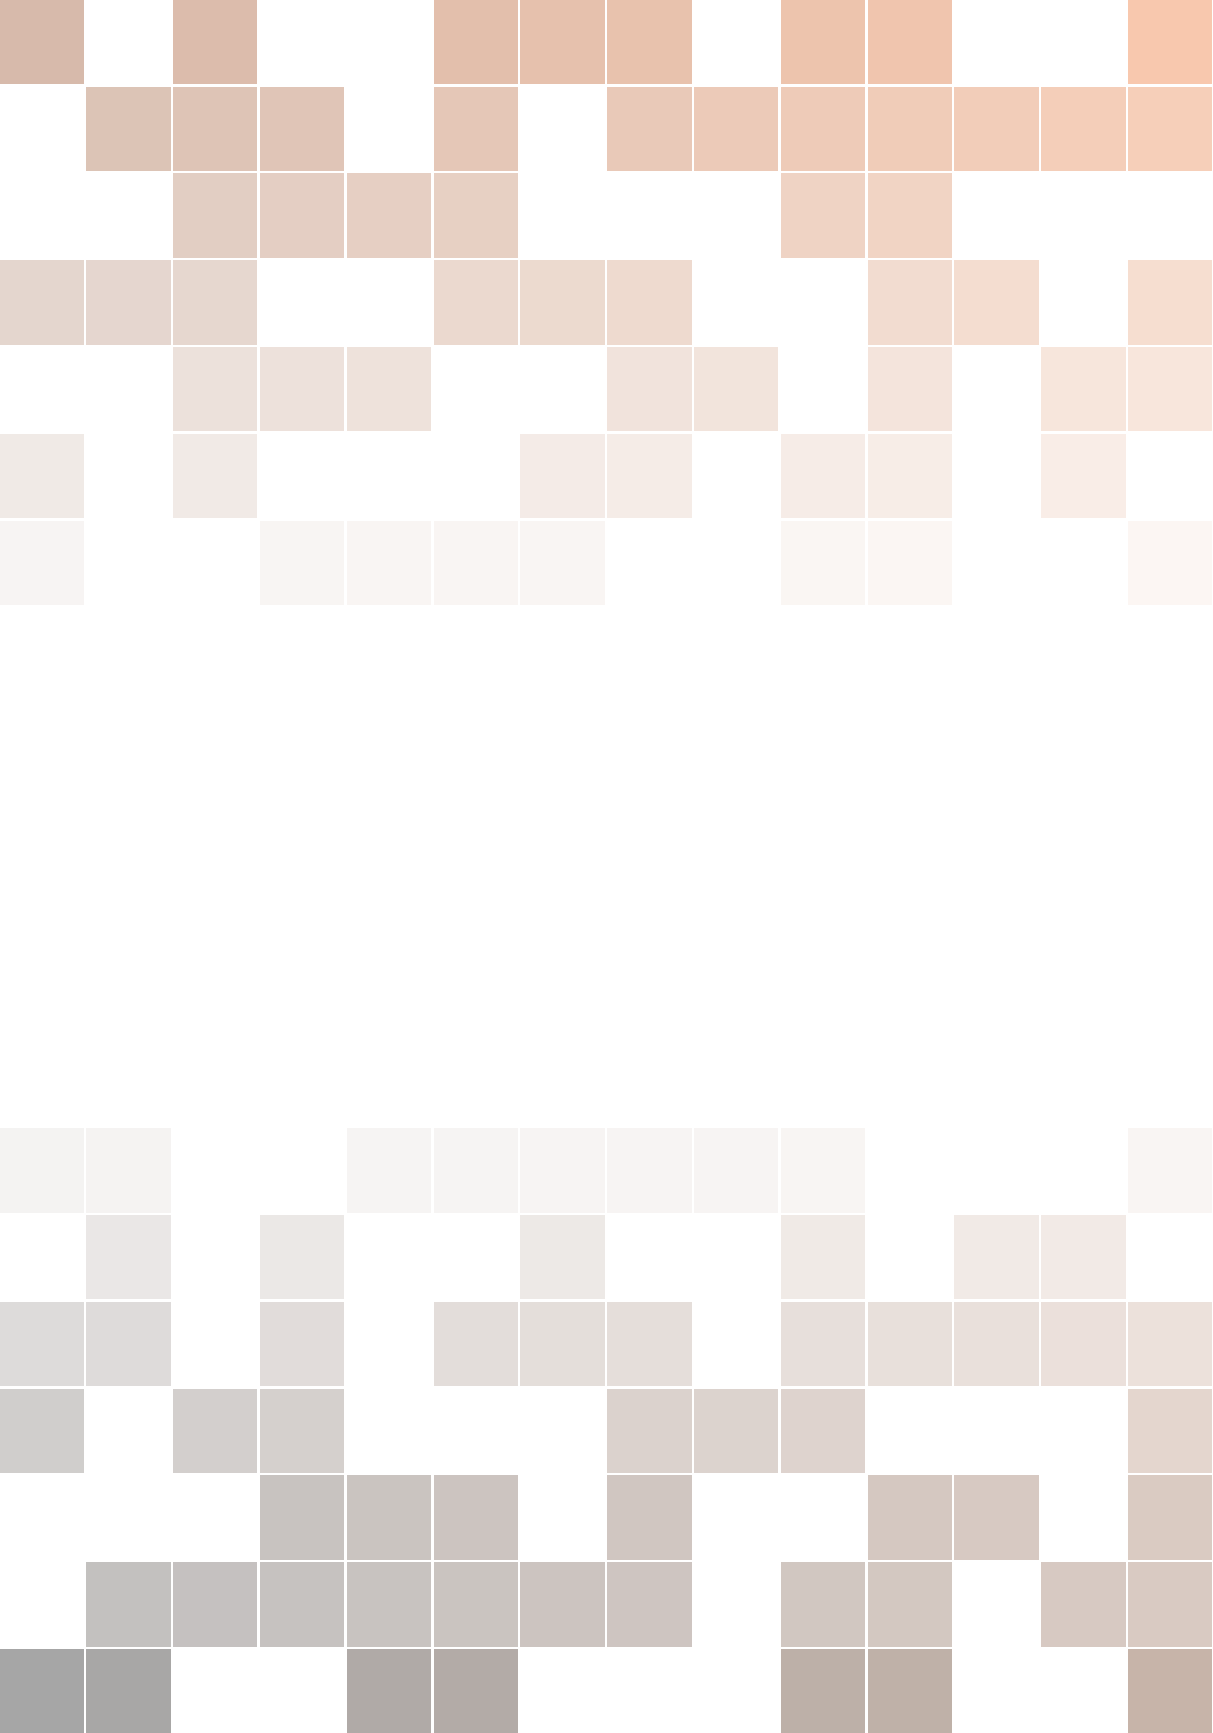
\includegraphics[scale=1]{background}}} % Image background
\centering
\vspace*{9cm}
\par\normalfont\fontsize{35}{35}\sffamily\selectfont
Dschungelbuch Siegen\\ {\LARGE Information für Menschen mit wenig Geld in und um Siegen}\par % Book title
\vspace*{1cm}
{\Huge Klaus Reifenrath}\par % Author name
\endgroup

%----------------------------------------------------------------------------------------
%	COPYRIGHT PAGE
%----------------------------------------------------------------------------------------

\newpage
~\vfill
\thispagestyle{empty}

\noindent Kein Copyright / no \copyright. Kopieren und Verteilen ausdrücklich erlaubt.\\ % Copyright notice

\noindent \textsc{Published by Klaus Reifenrath}\\ % Publisher

\noindent \textsc{www.krwe.de, klaus@krwe.de}\\ % URL

%\noindent Licensed under the Creative Commons Attribution-NonCommercial 3.0 Unported License (the ``License''). You may not use this file except in compliance with the License. You may obtain a copy of the License at \url{http://creativecommons.org/licenses/by-nc/3.0}. Unless required by applicable law or agreed to in writing, software distributed under the License is distributed on an \textsc{``as is'' basis, without warranties or conditions of any kind}, either express or implied. See the License for the specific language governing permissions and limitations under the License.\\ % License information

%\noindent \textit{First printing, March 2013} % Printing/edition date

%----------------------------------------------------------------------------------------
%	TABLE OF CONTENTS
%----------------------------------------------------------------------------------------

\chapterimage{chapter_head_1.pdf} % Table of contents heading image

\pagestyle{empty} % No headers

\tableofcontents % Print the table of contents itself

\cleardoublepage % Forces the first chapter to start on an odd page so it's on the right

\pagestyle{fancy} % Print headers again

%----------------------------------------------------------------------------------------
%	Vorwort
%----------------------------------------------------------------------------------------

\section{Vorwort von Klaus Reifenrath}

Informationen für Menschen in und um Siegen mit  wenig oder keinem Einkommen. Die Idee zum „Dschungelbuch Siegen“ ist mit Freunden und Betroffenen entstanden. Wir haben diese Informationen zusammengestellt und sie unter dem Namen \enquote{Dschungelbuch Siegen} im Internet veröffentlicht. Zu finden über Google \enquote{Dschungelbuch Siegen} oder unter \href{http://www.krwe.de}{ www.krwe.de}. Dort können Sie das \enquote{Dschungelbuch Siegen} kostenlos herunterladen, lesen oder ausdrucken und gerne an Menschen, die es interessiert, weitergeben. Es besteht kein Copyright und kein kommerzielles Interesse! Bitte weiterreichen. Es soll einfach nur eine Hilfe im Dschungel der Stadt darstellen. Wir suchen nach weiteren sozialen Einrichtungen in Siegen und Umgebung, damit wir das \enquote{Dschungelbuch Siegen} erweitern können. Senden Sie uns bitte per Mail eine Nachricht an \href{mailto:klaus@krwe.de}{klaus@krwe}, wenn Sie im \enquote{Dschungelbuch Siegen} etwas lesen, das sich geändert hat.

\section{Vorwort von nanooq}

Das Layout des Dschungelbuchs basiert \enquote{The Legrand Orange Book} von Mathias Legrand \href{mailto:legrand.mathias@gmail.com}{legrand.mathias@gmail.com} und steht unter \enquote{CC BY-NC-SA 3.0}. Das Dschungelbuch kam durch Uschi Shure über Esteban Shure an mich. Diese Version wird ebenfalls unter CC BY-NC-SA 3.0 im github-repository \href{https://github.com/nanooq/dschungelbuch-siegen}{https://github.com/nanooq/dschungelbuch-siegen} gehostet. Dort wird auch erklärt, wie man Einträge direkt aktualisieren kann. Weitergabe und Mitarbeit erwünscht. Danke an alle Hände und Köpfe, die mitmachen, ihr wisst, wer ihr seid. Viel Spaß beim Lesen und Verteilen!